\documentclass[12pt]{article}
\usepackage{mwe,tikz}\usepackage[percent]{overpic}
\pagestyle{empty}

\usepackage{latexsym}
\usepackage{dcolumn}
\usepackage{amsfonts,amssymb}
\usepackage{graphicx,epsfig}
\usepackage{psfrag}
\usepackage{amsmath,amssymb}
\usepackage{float}
\usepackage[normalem]{ulem} 
% \usepackage{showlabels}
% \usepackage[notref,notcite]{showkeys}
\usepackage{color}
\setlength\textwidth{16.9cm}
\setlength\textheight{22.35cm}
\addtolength\evensidemargin{0.2cm}
\addtolength\oddsidemargin{-1.9cm}
\setlength\topmargin{-0.6cm}
\setlength{\parskip}{1em}
\setlength{\parindent}{0em}

\def\be{\begin{equation}}
\def\ee{\end{equation}\noindent}
\def\ben{\begin{equation}}
\def\een{\end{equation}\noindent}
\def\ba{\begin{eqnarray}}
\def\ea{\end{eqnarray} \noindent}
\def\bea{\begin{eqnarray}}
\def\eea{\end{eqnarray} \noindent}
\def\nn{\nonumber}
\def\ni{\noindent}
\def\mco{\mathcal{O}}
\def\mcz{\mathcal{Z}}
\def\mcs{\mathcal{S}}
\def\mcR{\mathcal{R}}
\def\mcl{\mathcal{L}}
\def\mcn{\mathcal{N}}
\def\vv{{\bf v}}
\def\del{{\bf \nabla}}
\def\sech{\text{sech}}
\def\TT{\mathcal{T}}
\def\bz{{\bar{z}}}
\def\tq{{\tilde{q}}}
\def\RR{\mathcal{R}}
\def\emfg{\color{ForestGreen}}
\def\emb{\color{blue}}
\def\emr{\color{red}}
\definecolor{green}{rgb}{0,0.6,0.4}
\def\emg{\color{green}}
\def\emc{\color{cyan}}
\def\emo{\color{orange}}



\begin{document}

{\Large Ref:  LP15396}
 
 \vspace{20pt}

\centerline{\LARGE Universality of generalized parton distributions}

\vspace{5pt}
   
\centerline{\LARGE in light-front holographic QCD}
   
   

\vspace{10pt}

\centerline{Guy F. de T\'eramond, Tianbo Liu, Raza Sabbir Sufian,}

\centerline{Hans G\"unter Dosch,  Stanley J. Brodsky and Alexandre Deur}

\vspace{10pt}
 
\centerline{\today}

\vspace{30pt}
    
We are very grateful to the Referees for their careful review of our manuscript and providing many constructive comments. We have revised the manuscript according to the Referees' report and provide our response to their questions and comments below.

\section*{Reply to Referee A }

{\it The submitted manuscript presents a model ansatz for generalized
parton distributions (GPDs) in the valence sector, based on results
for nucleon form factors in light-front holographic QCD. The results
of this model are compared with other determinations of parton
distributions.} 

{\bf Reply:} We thank the referee for bringing up this discussion. In fact, it is the longitudinal reparametrization function $y = w(x)$ in the integral expression for the Euler Beta function in Eqs. (1) and (2), which is a priory unknown,  but is largely determined by the physical constraints imposed in the model.  A more detailed answer to this point is given in the reply to ``comment~2" below.  


{\it A strong point of the presented model is its relative simplicity, its
mathematical elegance, and the interesting feature that it connects
the forward $(t=0)$ limit of GPDs with their t-dependence via eqs (8)
and (9).On the other hand, the phenomenological reach of the model is
not completely clear to me, and the claim in the paper to provide
``precise descriptions of both the nucleon and the pion quark
distribution functions" is in my opinion problematic (see below). }


{\bf Reply:} We thank the Referee for the positive comments and we hope to address the Referee's concerns in our answers below. In particular we will confront the model results with extended sets of global fits: MMHT2014, CT14, and NNPDF3.0.


{\it I regard the present paper as a valuable contribution to the ongoing
effort of the community to formulate dynamically motivated models for
GPDs. However, I do not think that the work has the character of a
breakthrough or of a completely new idea, which would make it suitable
for publication in PRL. A publication in PRD seems much more
appropriate to me.}


{\bf Reply:} The comprehensive framework introduced in our work leads to connections previously unknown: Some of the analytic forms used extensively in the literature appear here as a consequence of the underlying analytic structure. The relation between the PDFs and the GPDs profile, which is arbitrary in other dynamical models, is here a necessity of the formalism. The formalism also leads to a nontrivial connection with Regge behavior incorporated in the expression for the Veneziano amplitude, which gives further insights into the understanding of quark-hadron duality and hadron  structure. Hence the structural framework introduced in this letter incorporates the interrelation of form factors  --independent of the specific form of $w(x)$, GPDs and the hadron spectrum from a completely new perspective. 



{\it Moreover, there are several issues in the paper which in my view
require clarification, before publication can be recommended. I now
discuss these in turn.}

{\it 1. \it The notion of ``twist" is used for form factors and associated
contributions to parton distributions (starting in eq 1). It is not
defined in the paper, and it clearly differs from the conventional
notion of ``twist" for parton distributions (all distributions
discussed here have twist 2 in the usual sense of the word). It is
therefore important to give a definition of the twist tau used here,
or to clearly refer to one paper where this information can be found.}

{\bf Reply:}  Twist $\tau$ here is the canonical dimension minus spin, $\tau = \Delta - \sigma$, where $\sigma$ is the sum over the constituents  spin, $\sigma = \sum_{i = 1}^n \sigma_i$: It is also equal to the number of constituents in a given Fock component in  the Fock expansion of a hadron state. It thus controls the short distance behavior of the hadronic state and thus the power-law asymptotic behavior of form factors and amplitudes as first shown in Refs.  [53] and [54]. We have added a proper definition of twist-$\tau$ used in the  manuscript to avoid confusion.

{\it Connected with this point, it remains unclear how the sums over
different twists arise in eqs (18,19), (20) and (22), and if these are
meant to be complete or truncated.}

{\bf Reply:} When computing a hadron form factor in light-front quantization one uses the Drell-Yan-West expression which is a sum over an infinite number of Fock states with different number of constituents, thus a sum of components with different twist.  Thus for example Eq. (20), which corresponds to Eq. (22) in the previous version,  reflects the fact that the space and time-like pion form factor is well described by twist-2 and twist-4 as shown in Ref. [28]. Eqs. (16), (17) and (18) for nucleons, which corresponds respectively to Eqs. (18), (19) and (20) in the previous version, also involve the orbital angular momentum which also contributes to light-front twist. One should, in principle, involve an infinite number of components in the Fock expansion,  but the results described in Refs. [28] and  [56] have shown that the truncated expansion, up to the subleading twist term, can already give quite reasonable descriptions of the pion and nucleon elastic form factors.


{\it 2. It is not clear to me whether the form (7) is meant to be a simple
ad-hoc ansatz (which has proved to be successful in the literature) or
whether it comes out of the light-front holographic QCD in an exact or
approximate way. Also, it remains unclear whether the use of a single
profile function $f(x)$ for all tau is meant to be a simplifying choice
or a necessity.}


{\bf Reply:} The form  Eq. (8), which corresponds to Eq. (7) in the previous version, is not an ansatz. It is derived from Eqs. (1) and (2),
\begin{align*}
H_\tau(x,t)&=\frac{1}{N_\tau}[1-w(x)]^{\tau-2}w(x)^{-\frac{t}{4\lambda}-\frac{1}{2}}w'(x)\\
&=\frac{1}{N_\tau}[1-w(x)]^{\tau-2}w(x)^{-\frac{1}{2}}w'(x)\exp\Big[\frac{t}{4\lambda}\log\Big(\frac{1}{w(x)}\Big)\Big],
\end{align*}
where $w(x)$ is the reparametrization function as defined in the manuscript. It can be rewritten into the form Eq. (8) with $q(x)$ and $f(x)$ defined in Eqs. (9) and (10). Although the form Eq.  (8) shares the same structure which appears in much of the GPD  literature, our results clearly show that Eqs.  (9) and (10) are not independent, but describe the connection  between the $x$-dependence and the $t$-dependence for the GPDs of arbitrary $\tau$. We have added  Eq. (6) to make this point clear. The universality of the profile function $f(x)$ is not a  simplifying choice but a strict result in the framework described here. Indeed,  the $\tau$ dependence is embedded in the form factor expressions in Eq. (1) and the Euler's canonical representation in Eq. (2). The reparametrization function $ w(x)$ in Eq. (6) is independent  of $\tau$.  This procedure keeps the universality of the analytical structure of GPDs.  We have written Eq. (8), previously Eq. (7), in a more explicit form in the revised version to clarify this point.


{\it Moreover, no motivation or derivation is given for the
requirement of the boundary values in eq (10).}

{\bf Reply:} The boundary conditions in Eq. (7), which corresponds to Eq. (10) in the previous version, are mathematical constraints, which follow from Euler's canonical representation of the Beta function in Eq. (2). The integral limit over $y$ is from $0$ to $1$, and the longitudinal momentum fraction $x$ in the reparametrization function $y=w(x)$ ranges from $0$ to $1$. These constraints require $w(0)=0$ and $w(1)=1$ with $w(x)$ monotonously increasing, or $w(0)=1$ and $w(1)=0$ with $w(x)$ monotonously decreasing. But the latter case is just an interchange of $x$ and $1-x$ from the former one, and it physically corresponds to an exchange of the active quark with the spectator. This has been clarified in the revised manuscript.


{\it 3. The relation (21) is not literally correct in that the r.h.s. gives
the ``valence" contribution from ``quarks minus antiquarks" to the
angular momentum, whereas Ji's sum rule holds for the contribution of
``quarks plus antiquarks". In this sense, comparison of the values for
$J^u$ and $J^d$ with lattice calculations is problematic when the latter
include contributions from disconnected lattice diagrams, which are
commonly associated with sea quark degrees of freedom. For some of the
published lattice results, it may be possible to compare with the
connected part, which is more valence like (although it does include $Z$
graph contributions and is hence not equivalent with ``quark minus
antiquark"). At least a warning should be given in the text.}

{\bf Reply:}  We thank the referee for this important comment. We now realize that a more extended discussion of this point is required if comparison with lattice results is included. On the other hand, this specific point does not shed much light on the new aspects of our model. We thus propose to eliminate from the present article Ji's sum rule and TABLE I and leave it for future discussion. 


{\it 4. I find the discussion of the large-$x$ behavior of the valence quark
distribution in the pion confusing in two respects. The authors write
that the $(1-x)$ behavior of their distribution corresponds to the
``pQCD inclusive hard counting rule". However, a detailed analysis of
the pQCD mechanism for the pion in Phys.Lett. B610 (2005) 247 (Ji et
al) gives $(1-x)^2$. Likewise, one obtains $(1-x)^2$ from Nucl.Phys. B441
(1995) 197 (Brodsky et al), although it is not clear whether the
formula for the $(1-x)$ power in that work is meant to be applicable for
spin-zero hadrons.}

{\bf Reply:}  The large-$x$ behavior for arbitrary twist $q_\tau(x) \sim (1-x)^{2 \tau -3}$ follows from the $x = 1$ boundary condition (13). 
This is the Drell-Yan inclusive counting rule from Ref. [61].  Therefore we have modified the text below Eq. (13) ``which is precisely the perturbative QCD (pQCD) inclusive hard counting rule for large-$x$'' by  ``which is precisely the Drell-Yan inclusive counting rule at $x \to 1$  corresponding to the form factor behavior  at large $Q^2$ (3).''  Notice that this is a natural result in the present framework, since the model incorporates the duality
$$ F_\tau(Q^2) \to \left(\frac{1}{Q^2}\right)^{2 \tau - 1}        \Longleftrightarrow ~~  q_\tau(x) \to (1-x)^{2 \tau - 3},$$
namely, the inclusive exclusive-inclusive connection from Ref. [61], which follows here from the boundary condition $w'(1) = 0$.

We notice that the introduction of quark masses leads to further suppression at the endpoints. We have added to the text:  ``Our analysis incorporates the nonperturbative behavior of effective LFWFs in the limit of zero quark masses. However, if we include a nonzero quark mass in the LFWFs [24, 84, 85] the PDFs will be further suppressed at $x \to 1$."

{\it Regarding the comparison between the evolved results of the present
model and QCD extractions of the pion PDF from data, I find it
insufficient to simply state that the model agrees with Refs [81,82]
but not with Ref [83] at high $x$. The analysis in Ref [83] clearly
shows that a reliable extraction of the large-$x$ PDFs from the
available data requires threshold resummation and that a fixed-order
approach as in [81,82] is unreliable there. In this sense, a mere call
for ``a new generation of experiments" as made in the conclusions also
seems somewhat unsatisfactory to me. (It would surely be good to have
new data, but one should also analyze the existing data with
appropriate theory.)}

{\bf Reply:} We will limit ourselves to point out the tension between  our nonpertubative results $1-x$ and the pQCD $(1-x)^2$ behavior and leave out the sentence ``which requires a new generation of experiments" from the conclusion.


{\it 5. I think that, apart from the issue just discussed, the results of
the model are in impressive agreement with other determinations of
PDFs, given the small number of parameters in the model ansatz.
However, to contrast this with ``the large number of parameters" in
global fits and models, as written in the abstract, is in my view
misleading because it suggests that the model can do as good with a
few parameters as other can with many. To uphold such a claim would
require a detailed quantitative analysis of how precisely the nucleon
valence PDFs are known (using a single PDF set for this is known to be
insufficient as the discrepancies between PDF sets are typically
larger than their respective error bands). A similar comment holds for
the description of nucleon form factors, which in some regions are
measured to percent accuracy whilst in other regions different data
sets are clearly incompatible within their quoted errors. How
precisely the model results of the paper describe these quantities
within their true uncertainties is not quantified in the paper.}

{\bf Reply:} Following the referee's suggestion, we have removed ``the large number of parameters" from the text and amended the sentence in the abstract as  ``A simple ansatz for $w(x)$ which fulfills these physics
constraints with a single-parameter results in precise descriptions of both the nucleon and the pion
quark distribution functions in comparison with global fits." We have also slightly modified the abstract.

We  compare in Figure~\ref{proton_more} our results with the MMHT2014 and the CT14 sets in addition to the NNPDF3.0 set that has been included in the manuscript. The new figure gives a better idea of how well the the nucleon PDFs are known and has been updated in the manuscript.

\begin{figure}[!h]
\centering
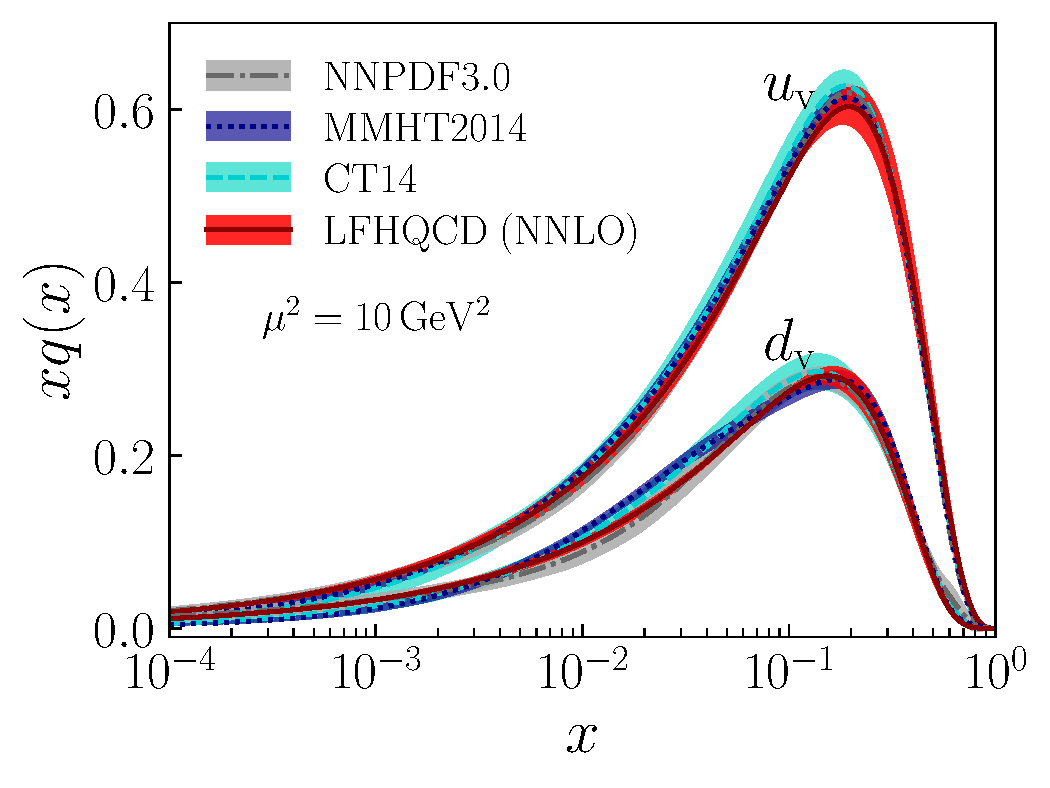
\includegraphics[width=0.6\textwidth]{proton-more-xf.pdf}
\caption{Comparison of nucleon PDF results with different global fit PDF sets. The red bands are the LFHQCD results. The gray bands are NNPDF3.0 fit, the blue bands are MMHT2014 fit, and the cyan bands are CT14 fit. \label{proton_more}}
\end{figure}
\begin{figure}[!h]
\centering
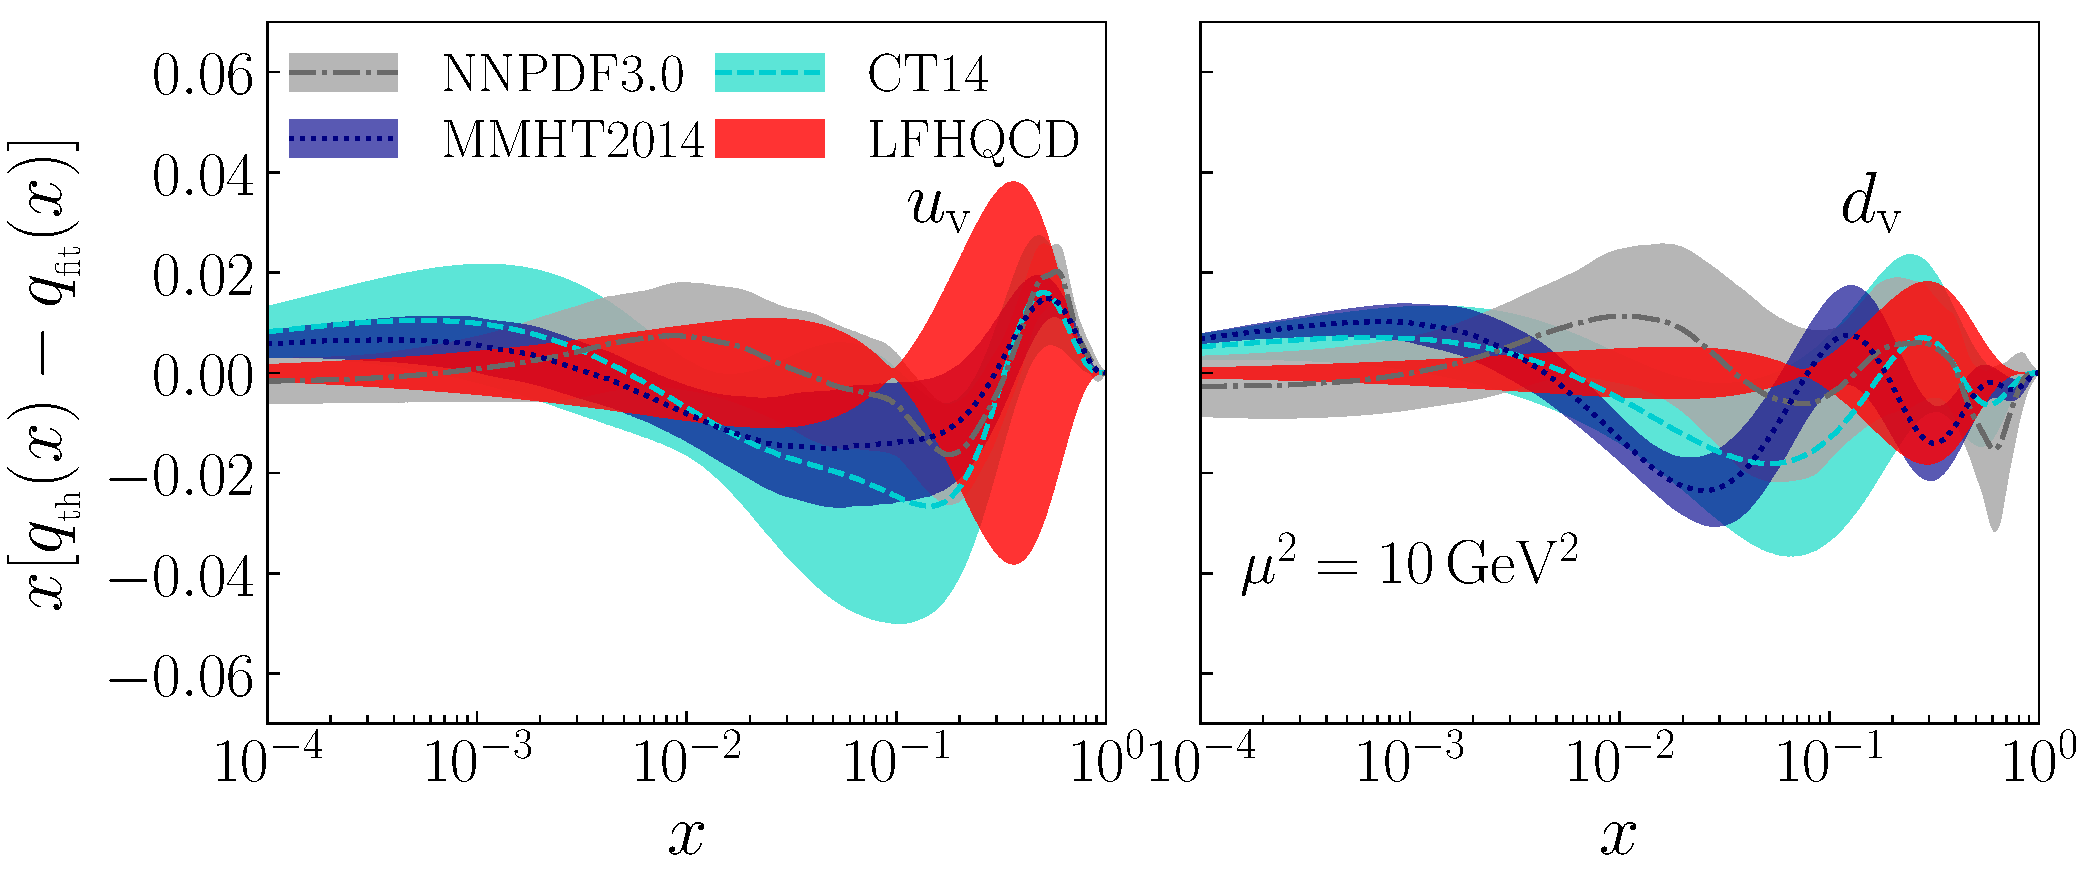
\includegraphics[width=0.85\textwidth]{proton-diff-xq.pdf}
\caption{The difference between nucleon PDFs calculated from LFHQCD (red band) and those from global fits for $u_{\rm v}$ (left) and $d_{\rm v}$ (right) from NNPDF3.0 (grey), MMHT2014 (blue), and CT14 (cyan).\label{proton_diff}}
\end{figure}

Furthermore, to quantify the difference between our results and the global fits, we show the difference in Figure~\ref{proton_diff}. We have included it as Fig. 3 in the updated version of the manuscript.


{\it If the above points can be clarified, the manuscript should be very
suitable for publication as a regular article in PRD.}


{\bf Reply:}  We believe that our responses above, together with the updated manuscript, clearly demonstrate  that the comprehensive structural framework introduced here, its simplicity, universality, and  possible extensive applications, constitutes a significant advance in an important field, which makes this work suitable for publication in PRL.



\newpage


\section*{Reply to Referee B}

{\it The authors discuss the general expression for the generalized parton
distributions (GPDs) of pions and nucleons derived from light-front
holographic QCD.}

{\it The remarkable result of this work is the possibility to provide a
consistent description of both the hadron spectrum, and exclusive and
inclusive observables within an unitary framework.}

{\it Generalized parton distributions are a new type of functions which
contain all the physics encoded in form factors and ordinary parton
distributions. In this paper, GPDs are derived using an integral
relation with the hadron form factors, that have been calculated in
previous works by some of the authors using light-front holographic
QCD. The results for the valence-quark GPDs are obtained in terms of
an universal function, for both pions and nucleons, which is
constrained by boundary conditions fixed in terms of physical
arguments dictated from the behavior of the collinear parton
distribution functions (PDFs) at large and small x.}

{\it The results for the valence-quark PDFs reproduce very well the
behavior of existing phenomenological parametrizations. Predictions
for the GPDs as function of x and different values of t are also
shown. The results of this analysis are very interesting, and
represent a step forward with respect to existing works ``inspired" by
light-front holography, but often introducing a number of free
parameters with poor contacts with the original theory.}

{\it For these reasons, I believe that the paper is worth to be published.}

{\bf Reply:} We thank the Referee for encouraging comments and  recommendation for the publication in PRL. We address the recommendations below.

{\it However, I would recommend the authors the following improvements:}

{\it 1) the relation between the form factors and the unpolarized GPDs
written just above Eq. (7) is valid only for the valence-quark GPDs,
otherwise the integral of $H^q$ should run between [-1,1] (see for
example, Eqs. (7) and (8) of Ref. [66]);}

{\bf Reply:} We thank the referee for pointing this out. To avoid confusion we have consistently added a subscript  ``$\rm v$" in all the relevant formulas.


{\it 2) the definition of twist which is used throughout the paper is
different from the standard definition of twist used to classify the
PDFs and GPDs. The authors should clarify this point, starting from
Eq. (8), to avoid misunderstandings;}


{\bf Reply:}  Twist $\tau$ refers here to the canonical dimension minus twist of each Fock component in the Fock expansion of a hadron state: it is the number of constituents of a given Fock component.  It determines the asymptotic behavior of form factors. We have clarified this point in the manuscript.


{\it 3) in Fig. 1 the results for the nucleon PDFs are compared with the
parameterization of Ref. [75] at NNLO, while the results for the pion
PDFs are given at NLO. Did the author check the convergence of the
perturbative evolution by comparing also the results for the nucleon
PDF with phenomenological parametrizations for the nucleon PDFs at
NLO?}

{\bf Reply:} Following the Referee's suggestion, we show the comparison between our nucleon PDF results evolved at NLO and the NLO phenomenological parametrization (NNPDF3.0) in Figure~\ref{proton_nlo}. The uncertainty bands are understood in the same way as those in the manuscript. The initial evolution scale is set accordingly as described in the text for the pion PDF.

\begin{figure}[!h]
\centering
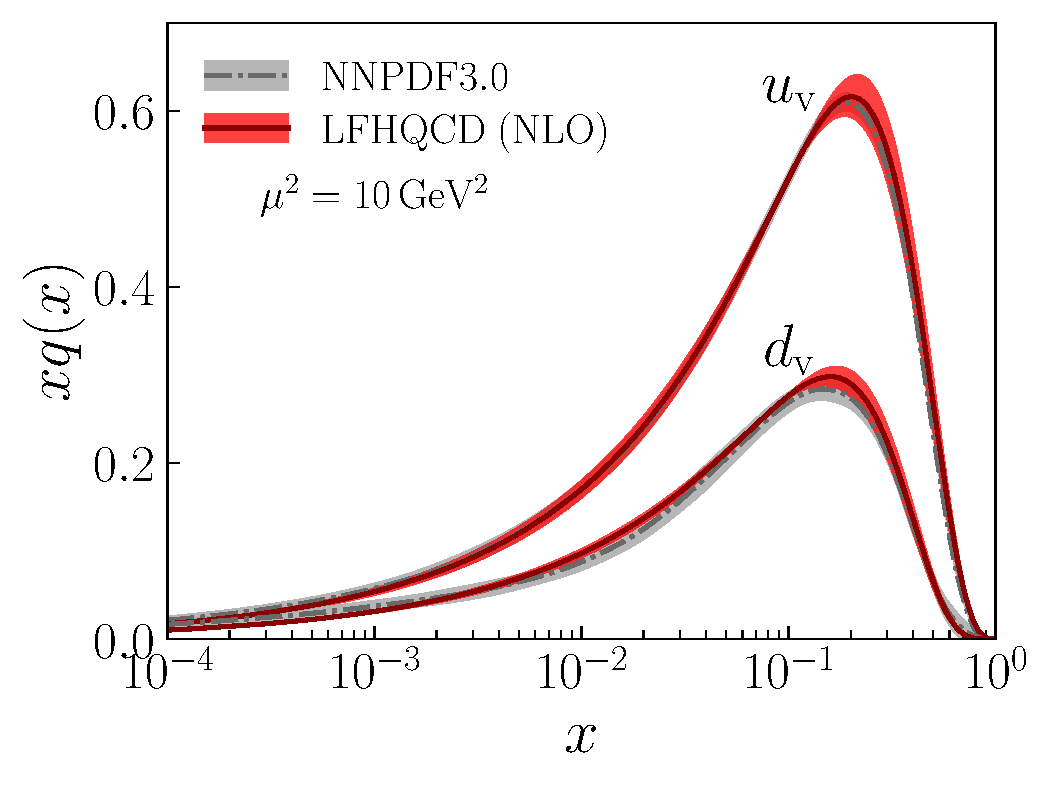
\includegraphics[width=0.6\textwidth]{proton-NLO-xf.pdf}
\caption{The nucleon PDFs in comparison with the global  NNPDF3.0 analysis at NLO.\label{proton_nlo}}
\end{figure}

As can be observed from the figure, the agreement for the NLO results is as good as that for the NNLO results, which have been presented in the manuscript, in comparison with global fits. 

{\it 4) it would be convenient to explicitly write at the end of page 2 the
numerical value of $\lambda$ taken from Ref. [28] and the numerical
value of $A^q(0)$ introduced at the end of page 3;}

{\bf Reply:} We have added the numerical value of $\lambda$ on page 2, below Eq. (5), and added a new reference [57] where the uncertainties in $\lambda$ are discussed. The value $a=0.507 \pm 0.034$ was determined from the first moment of the GPD, $\int_0^1 dx\, xH_{\rm v}^q(x,t=0)=A_{\rm v}^q(0)$ from a NNPDF3.0 NNLO fit with $A_{\rm v}^u(0)=0.259\pm0.004$ and $A_{\rm v}^d(0)=0.108\pm0.005$ at $\mu^2=10\,{\rm GeV}^2$.  Moreover, in the present version we extend the model comparison with the MMHT2014, CT14 in addition to the NNPDF3.0 global data  fit. We have thus determined the value of the parameter $a$ and its uncertainty by minimizing the sum rule from the extended data sets.  The new value from the global data fit average is $a = 0.531 \pm 0.037$. This is described on page 3.


{\it 5) in the caption of Fig. 2, it should be written the scale $\mu^2$ to
which the results refer. It would also be interesting to compare the
results with phenomenological studies for the GPDs obtained in a
similar way from the study of the electromagnetic form factors, like
for example in Ref. [66] (for example, in Ref. [66] the fit ABM 0
refers to the scale $\mu^2=1$ GeV$^2$ which is similar to the scale of
the present work);}

{\bf Reply:} We have added the scale $\mu_0$ in the captions of  Fig. 3 and Fig. 5, which correspond to Figs. 2 and 4 in  the previous version. We have also added the initial scale in the captions of Fig. 1 and Fig. 4.  Due to PRL space constraints, we leave the more extended discussions and comparisons with phenomenological fits for GPDs for future studies.


{\it 6) analogously, it would be instructive to compare the results for the
pion GPDs in Fig. 3 with existing light-front model calculations.}

{\bf Reply:}    Due to PRL space constraints, we leave the more extended discussions and the comparison between the present model results with other pion GPD models for future studies.


{\it 7) in the introduction of page 1, the authors refer to the analytic
form of GPDs found in Ref. [53]. However, I could not find any
analytic form for the GPDs in the cited paper, which, instead,
contains the calculation of the pion electromagnetic form factor.
Could the author specify better to which expression they refer?}

{\bf Reply:} We refer to Eq. (D.5) in the Appendix of this reference,  which is now Ref. [52] in the revised version. It is interesting to note that this early attempt to extract a parton distribution from holographic QCD corresponds to $w(x) = x$ in the present framework. The expression (D.5) is  limited in two respects: a) it does not incorporate the correct $x^{-1/2}$ small-$x$ Regge behavior (which comes from the correct pole positions of the $\rho$ and its radial excitations and b) although $w(x) = x$ satisfies trivially the constraints $w(0) = 0$ and $w(1) = 1$, it does not satisfy the condition $w'(1) = 0$. Therefore it does not include the Drell-Yan exclusive-inclusive connection.


{\it 8) also, I find improper to include Ref. [36] in the list of
references [30-52] cited in the introduction, in the second paragraph
of the second column. As a matter of fact, the quark spectator model
used in the work of Ref. [36] is not taken from LFHQCD.}

{\bf Reply:} We have removed Ref. [36] form the list of references.


{\it 9) I also did not find the corresponding references when speaking
about ``our previous results for GPDs", in the last paragraph of the
introduction.}

{\bf Reply:} The previous expression for the GPDs discussed in our reply to  point 7) is given in (D. 5) of Ref. [52], which corresponds to Ref. [53] in  the previous version, and the effective LFWFs by Eqs. (A. 20) and (A. 21) of  Ref. [55], which corresponds to Ref. [56] in  the previous version. As we mention in the article, the $x$-dependence for the expressions for the parton distributions and effective LFWFs are  modified.

{\it 10) note that the appendix on page 5 is never quoted in the main text
of the manuscript.}

{\bf Reply:} We have moved the contents of the appendix to the main text.

Finally, we hope that we have answered the questions by the Referees in a proper and systematic way. We appreciate the comments and suggestions by the Referees whose inclusions have noticeably improved the draft.


\end{document}